\documentclass{article}
\usepackage[utf8]{inputenc}
\usepackage{hyperref}
\usepackage{listings}
\usepackage{color}
\usepackage{amsmath}
\usepackage{amsfonts}
\usepackage{sourcecodepro}
\usepackage{xcolor}
\usepackage[]{minted}
\usepackage[utf8]{inputenc} % Required for inputting international characters
\usepackage[T1]{fontenc} % Output font encoding for international characters
\usepackage{tikz}
\usetikzlibrary{angles,quotes}
\usepackage{float}
\usepackage{tikz-3dplot}

\lstdefinestyle{CStyle}{
    backgroundcolor=\color{backgroundColour},   
    commentstyle=\color{mGreen},
    keywordstyle=\color{magenta},
    numberstyle=\tiny\color{mGray},
    stringstyle=\color{mPurple},
    basicstyle=\footnotesize,
    breakatwhitespace=false,         
    breaklines=true,                 
    captionpos=b,                    
    keepspaces=true,                 
    numbers=left,                    
    numbersep=5pt,                  
    showspaces=false,                
    showstringspaces=false,
    showtabs=false,                  
    tabsize=2,
    language=C
}

\begin{document}
\begin{titlepage} % Suppresses displaying the page number on the title page and the subsequent page counts as page 1
	
	\raggedleft % Right align the title page
	
	\rule{1pt}{\textheight} % Vertical line
	\hspace{0.05\textwidth} % Whitespace between the vertical line and title page text
	\parbox[b]{0.75\textwidth}{ % Paragraph box for holding the title page text, adjust the width to move the title page left or right on the page
		
		{\Huge\bfseries Quake's Player \\[0.5\baselineskip] Movement}\\[2\baselineskip]
		{\large\textit{A Breakdown Of Its Code \& Ramblings}}\\[4\baselineskip]
		{\Large\textsc{mia ivy}}
		
		\vspace{0.5\textheight}
        {\noindent Version 4, September 2023}\\[\baselineskip]
		
		}

\end{titlepage}
\tableofcontents
\newpage
\part{Velocity \& Acceleration}
\section{PM\_AirMove}
\texttt{PM\_AirMove}, despite its name, mainly handles finding the direction that the player should be moved in. Our player presses some input keys, and is facing a certain direction, and this function mainly
does some math to construct a vector that points in the direction we intend to move the player in. So, how do we do this? Let us take a look at Quake’s implementation:
\begin{minted}[linenos,tabsize=2,breaklines,firstnumber=512]{c}
	fmove = pmove.cmd.forwardmove;
	smove = pmove.cmd.sidemove;
	
	forward[2] = 0;
	right[2] = 0;
	VectorNormalize (forward);
	VectorNormalize (right);
\end{minted}
    
So, starting at the beginning, we obtain values $\texttt{smove}$ and $\texttt{fmove}$, which are values provided based on user input (the WASD keys). Then, we obtain the 3D vectors $\texttt{forward}$ and $\texttt{right}$. $\texttt{forward}$ is the vector that points in the direction the player is looking, and $\texttt{right}$ is the vector orthogonal to $\texttt{forward}$ on the $xy$-plane (there is also the vector $\texttt{up}$, orthogonal to both). We only care about the direction $\texttt{forward}$ and $\texttt{right}$ point in the $xy$-plane, so we remove their $z$-coordinate, and then we must re-normalize them as removing this coordinate does not leave us with a normalized vector. 
\begin{minted}[linenos,tabsize=2,breaklines,firstnumber=520]{c}
	for (i=0 ; i<2 ; i++)
		wishvel[i] = forward[i]*fmove + right[i]*smove;
	wishvel[2] = 0;

	VectorCopy (wishvel, wishdir);
	wishspeed = VectorNormalize(wishdir);
\end{minted}
Then, we sum these two vectors, with each vector in the sum scaled by the cvar associated with it. This makes sure that if one cvar, say the $\texttt{cl\_sidespeed}$ cvar, is smaller than $\texttt{cl\_forewardspeed}$, it will contribute a smaller portion to this vector we are calculating. We then nuke the $z$-coordinate, just in case. Lastly, we copy $\texttt{wishvel}$ into $\texttt{wishdir}$, and we set $\texttt{wishspeed}$ to be the length of $\texttt{wishdir}$, and then normalize the vector. Thus, we have a value for the magnitude of our speed, and our intended direction. 
\begin{minted}[linenos,tabsize=2,breaklines,firstnumber=527]{c}
//
// clamp to server defined max speed
//
	if (wishspeed > movevars.maxspeed)
	{
		VectorScale (wishvel, movevars.maxspeed/wishspeed, wishvel);
		wishspeed = movevars.maxspeed;
	}  
\end{minted}
We now wish to check that our speed is within appropriate bounds. This piece of code simply checks if $\texttt{wishspeed}$ exceeds our defined maximum speed, and if so, it scales $\texttt{wishvel}$ by $\frac{\texttt{movevars.maxspeed}}{\texttt{wishspeed}}$, and sets $\texttt{wishspeed}$ to be the maximum speed value. 
\begin{minted}[linenos,tabsize=2,breaklines,firstnumber=539]{c}
	if ( onground != -1)
	{
		pmove.velocity[2] = 0;
		PM_Accelerate (wishdir, wishspeed, movevars.accelerate);
		pmove.velocity[2] -= movevars.entgravity * movevars.gravity * frametime;
		PM_GroundMove ();
	}
\end{minted}
Now, we check if we are grounded. If we are, we set our velocity’s $z$-component to be 0, then we pass on $\texttt{wishdir}$, $\texttt{wishspeed}$, and $\texttt{movevars.accelerate}$ to the function $\texttt{PM\_Accelerate}$, which handles acceleration on the ground. We then apply gravity, although this does not really have an effect since we are grounded. Lastly, we move our player with a call to the $\texttt{PM\_GroundMove}$ function.
\begin{minted}[linenos,tabsize=2,breaklines,firstnumber=546]{c}
else
	{	// not on ground, so little effect on velocity
		PM_AirAccelerate (wishdir, wishspeed, movevars.accelerate);

		// add gravity
		pmove.velocity[2] -= movevars.entgravity * movevars.gravity * frametime;

		PM_FlyMove ();

	}
\end{minted}
If we are not grounded, we simply pass the same information the the $\texttt{PM\_AirAccelerate}$ function instead, also append gravity to the z-coordinate of our velocity, and then move our player using the $\texttt{PM\_FlyMove}$ function.
\section{PM\_Accelerate}
We want our player to accelerate in a nice fashion, and doing so is a little bit different than what you may imagine. Simply taking our intended direction vector scaled and adding a small portion of it to our current velocity every frame, with checks for a maximum velocity, will not yield nice feeling movement. Turning feels especially disgusting, and it does not respond very nicely to how we change our view angle as we move about. To make moving less awful, we want to give some leniency in exceeding the maximum velocity limit when turning. In particular, we want to give more leniency the more you turn, and enforce a more strict limit otherwise. This is how Quake chose to implement this idea:
\begin{minted}[linenos,tabsize=2,breaklines,firstnumber=400]{c}
	currentspeed = DotProduct (pmove.velocity, wishdir);
	addspeed = wishspeed - currentspeed;
	if (addspeed <= 0)
		return;
	accelspeed = accel*frametime*wishspeed;
	if (accelspeed > addspeed)
		accelspeed = addspeed;
	
	for (i=0 ; i<3 ; i++)
		pmove.velocity[i] += accelspeed*wishdir[i];	
\end{minted}
First, we take the magnitude of our current velocity in the direction of $\texttt{wishdir}$, and store this as $\texttt{currentspeed}$. Then, we subtract this from $\texttt{wishspeed}$. This means that if we have a component of our velocity in the direction of $\texttt{wishdir}$ that exceeds the cvar set max speed, this difference will be 0 or negative. If this difference is 0 or negative, we do not accelerate the player, and simply return. \\
\begin{figure}[!ht]
\centering
    \begin{tikzpicture}[scale=0.9]
    \hspace{-3.25cm}
        \draw[thin,gray!40] (-1,-1) grid (6,6);
        \draw[<->] (-1,0)--(6,0) node[right]{$x$};
        \draw[<->] (0,-1)--(0,6) node[above]{$y$};
        \draw[line width=2pt,blue,-stealth](0,0)--(0,6)
        node[midway,above=0.1cm,sloped]{$vel$};
        \draw[line width=2pt,red](2.9,2.9)--(6,6) node[midway,above=-0.5cm,sloped]{$wishdir$};
        \draw[line width=2pt,red](0,0)--(-1,-1);
        \draw[line width=2pt,black,dashed](0,6)--(3,3);
        \draw[line width=2pt,black,-stealth](0,0)--(3,3)
        node[midway,above=-0.6cm,sloped]{$wishdir(\Vert vel \Vert\cos{\theta})$};
        \draw[black,dashed] (1,1) arc (45:90:1.44)node[midway,above=0.1cm]{${\theta}$};
        \node at (2.5,-1.5) {\textit{$\theta=45^{\circ}$}};
    %\end{tikzpicture}
    \hspace{7cm}
    %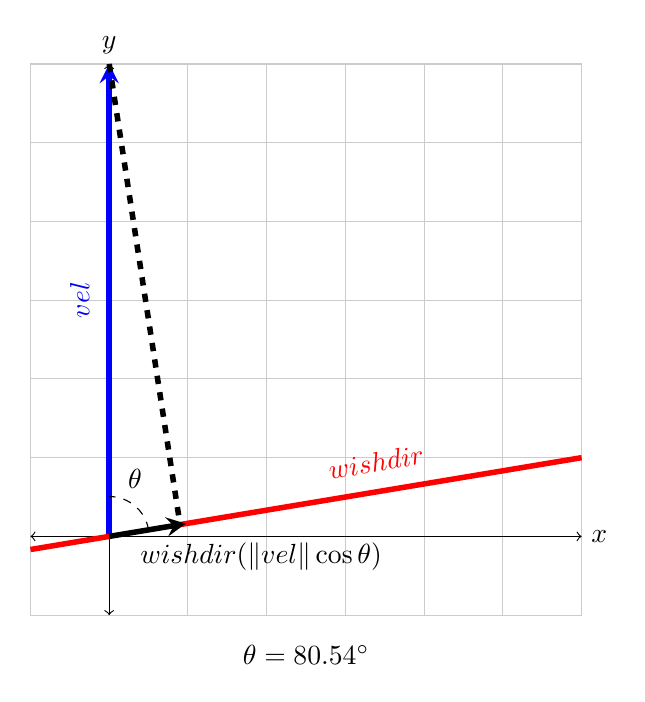
\begin{tikzpicture}
        \draw[thin,gray!40] (-1,-1) grid (6,6);
        \draw[<->] (-1,0)--(6,0) node[right]{$x$};
        \draw[<->] (0,-1)--(0,6) node[above]{$y$};
        \draw[line width=2pt,blue,-stealth](0,0)--(0,6)
        node[midway,above=0.1cm,sloped]{$vel$};
        \draw[line width=2pt,red](0.9,0.15)--(6,1) node[midway,above=0.1cm,sloped]{$wishdir$};
        \draw[line width=2pt,red](0,0)--(-1,-1/6);
        \draw[line width=2pt,black,dashed](0,6)--(0.9,0.15);
        \draw[line width=2pt,black,-stealth](0,0)--(0.9727,0.162)node[near start,above=-0.3cm,right]{$wishdir(\Vert vel \Vert\cos{\theta})$};
        \draw[black,dashed] (1/2,1/12) arc (9.46:90:1.014/2)node[midway,above=0.1cm]{$\theta$};
        \node at (2.5,-1.5) {\textit{$\theta=80.54^{\circ}$}};
    \end{tikzpicture}
    \caption{Projection of $vel$ onto the line spanned by $wishdir$. The length of this projection is $currentspeed$. If this length exceeds $wishspeed$, we do not accelerate} \label{fig:M1}
\end{figure}
Now, we find a constant $\texttt{accelspeed}$ by scaling $\texttt{wishspeed}$ by an acceleration constant, and factoring in the time since last frame. If this is larger than $\texttt{addspeed}$, then we set it to be $\texttt{addspeed}$ instead. From here, we scale each component of $\texttt{wishdir}$ by $\texttt{accelspeed}$ and add it to our velocity.  \\
\\
This short implementation has some interesting consequences. For one, it does what we intend. If we begin with no velocity and simply hold w, we accelerate until our velocity has a component in the direction of $\texttt{wishdir}$ that is as big as or exceeds the cvar set speed. As we are only moving straight forward, we stop accelerating exactly when our velocity is the max set velocity, which is what we want. From here, if we decide to turn to one side, we obtain a smaller component of our velocity in the direction of $\texttt{wishdir}$, and the more drastically we turn the smaller this component is. However, as we build speed by accelerating, this means that our overall velocity vector will gradually have a larger component in the direction of $\texttt{wishdir}$ unless they are orthogonal, meaning that as we build speed we have a smaller range of $\texttt{wishdir}$ angles that will give us this extra acceleration. This consequence is what we call (air)strafing. 

\section{PM\_AirAccelerate}
This function acts very similarly to $\texttt{PM\_Accelerate}$:
\begin{minted}[linenos,tabsize=2,breaklines,firstnumber=422]{c}
	if (wishspd > 30)
		wishspd = 30;
	currentspeed = DotProduct (pmove.velocity, wishdir);
	addspeed = wishspd - currentspeed;
	if (addspeed <= 0)
		return;
	accelspeed = accel * wishspeed * frametime;
	if (accelspeed > addspeed)
		accelspeed = addspeed;
	
	for (i=0 ; i<3 ; i++)
		pmove.velocity[i] += accelspeed*wishdir[i];	
}
\end{minted}

The main difference here is that our $\texttt{wishspeed}$ is restricted to being within the bounds of 0 to 30, instead of our usual value (which is 400 by default for Quake). Thus, we only accelerate up to a tiny velocity if we hold w from rest (in the $xy$-plane) while airborne. This also means that we have a significantly reduced range of $\texttt{wishdir}$ angles to gain speed with, and requires us to be very close to $90^{\circ}$ to gain any extra acceleration. 

\section{PM\_Friction}
This function handles friction. It is pretty straight forward, so this section will be brief.
\begin{minted}[linenos,tabsize=2,breaklines,firstnumber=336]{c}
	vel = pmove.velocity;
	
	speed = sqrt(vel[0]*vel[0] +vel[1]*vel[1] + vel[2]*vel[2]);
	if (speed < 1)
	{
		vel[0] = 0;
		vel[1] = 0;
		return;
	}
\end{minted}
To begin, we check if our speed is less than 1. If so, we simply come to a rest. This prevents friction from reducing our velocity with an asymptote where we never actually end up with 0 velocity, just an increasingly negligible small float number.
\begin{minted}[linenos,tabsize=2,breaklines,firstnumber=348]{c}
// if the leading edge is over a dropoff, increase friction
	if (onground != -1) {
		start[0] = stop[0] = pmove.origin[0] + vel[0]/speed*16;
		start[1] = stop[1] = pmove.origin[1] + vel[1]/speed*16;
		start[2] = pmove.origin[2] + player_mins[2];
		stop[2] = start[2] - 34;

		trace = PM_PlayerMove (start, stop);

		if (trace.fraction == 1) {
			friction *= 2;
		  }
    }
\end{minted}
This section simply determines if we are about to drop off of a ledge using a trace, which we will discuss later. If we find that we are about to move near a ledge, we double friction. The ledge needs to be at most a 34 unit drop for this to be taken into account.
\begin{minted}[linenos,tabsize=2,breaklines,firstnumber=364]{c}
if (waterlevel >= 2) // apply water friction
		drop += speed*movevars.waterfriction*waterlevel*frametime;
	else if (onground != -1) // apply ground friction
	{
		control = speed < movevars.stopspeed ? movevars.stopspeed : speed;
		drop += control*friction*frametime;
	}
\end{minted}
Now, we want to figure out how much to drop our velocity. Barring the water case because moving in water is fucking lame and we don't care about it, we find a variable $\texttt{control}$ through the use of a ternary operator. If our speed is less than some minimum stop speed (this is 100 in Quake by default), then we use the stop speed, otherwise we continue using our speed. Then, we find the amount to drop our velocity as this result scaled down by friction, and our frame time factored in. 
\begin{minted}[linenos,tabsize=2,breaklines,firstnumber=373]{c}
// scale the velocity
	newspeed = speed - drop;
	if (newspeed < 0)
		newspeed = 0;
	newspeed /= speed;

	vel[0] = vel[0] * newspeed;
	vel[1] = vel[1] * newspeed;
	vel[2] = vel[2] * newspeed;
}
\end{minted}
We find the difference between our current speed and the amount by which we intend to drop. If this is negative, we set our $\texttt{newspeed}$ to 0. Otherwise, we find the ratio of this $\texttt{newspeed}$ to our old speed, and scale our velocity by this amount.
\newpage
\part{The Ungodly Prison That Is Collisions}
\section{Motivation}
One big topic that is needed for any proper movement system is collisions. We want to know if we collide with something, and we also want to know information about the collision, and then what we want to do with this information. Generally, the information you need is if you collided or not, the depth of the collision, and the normal of the plane you collided with. Provided this information, we can accurately behave how we should when colliding with walls and floors. The reason we want this information is that we do not simply want to stop moving if we collide. If this were the case, hitting a wall at any angle or simply touching the floor would prevent us from moving. We instead want to remove the component of our velocity that is in the direction of the normal of collision. This way, when you touch ground, only gravity is removed from your velocity, thus, you stand on the object. If you walk into a wall at an angle, only the component of your velocity that is normal/perpendicular to the wall will be removed, meaning you will slide along the wall at a slower speed. It should also be noted that later into Quake's code, there is a check to see the slope of the plane you collide with below your player exceeds some magic number, and if so, we are simply considered airborne. The consequence of this check with properly implemented collisions and airstrafe is what is known as surf.
\section{GJK Algorithm In A Nutshell}
One popular collision algorithm that provides us a good start in detecting collisions is the Gilbert-Johnson-Keerthi algorithm, or GJK for short. This algorithm simply tells us "yes" or "no" for if we collide, but it is possible to write a more complex version of this algorithm that provides more detail. At its core, the GJK algorithm relies on an interesting observation: if we think about two shapes as simply an infinite collection of points that occupy the space of the shape, then we can do operations on these points. We can subtract the coordinates of each point in one shape from the other and generate a new shape, for example. In particular, it is interesting to note that if two shapes collide, then there exists some point inside one shape that is now also in the same coordinate position as a point in the other shape. Thus, the difference of the coordinates will be 0 (the origin).\\
\begin{figure}[H]
    \centering
    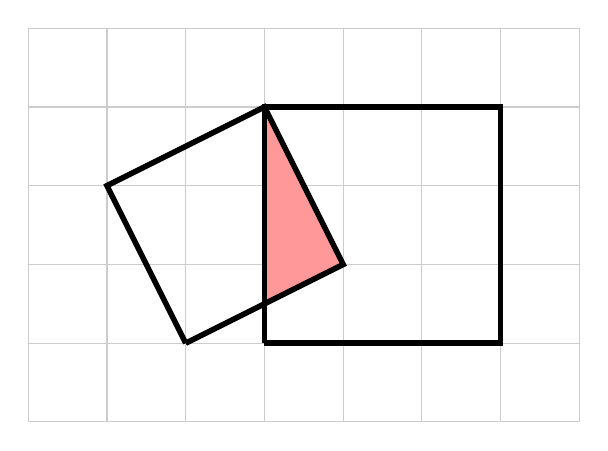
\begin{tikzpicture}
        \draw[thin,gray!40] (0,0) grid (7,5);
        \fill[red!40!white](3,1.5) -- (4,2) -- (3,4) -- (3,1.5);
        \draw[line width=2pt,black](2,1) -- (1,3)--(3,4)--(4,2)--(2,1);
        \draw[line width=2pt,black](3,1) -- (3,4)--(6,4)--(6,1)--(3,1);
    \end{tikzpicture}
    \caption{Two overlapping polygons. They share points with the same coordinates in the shaded region, which results in a Minkowski Difference containing the origin}
\end{figure}
This is the basis for GJK. We take two convex shapes, generate a shape by subtracting the points in one shape from another (which is usually called the Minkowski Difference), and if this new shape contains the origin, then the two original shapes must intersect. However, it is infeasible to compute the Minkowski Difference with an infinite number of points, and so instead we can simply work with the vertices of the shapes. We subtract each vertex of one shape from every other vertex of the other shape, and get a huge number of coordinates, most of which we actually do not care about. We only care about the "outer-most" coordinates of this Minkowski Difference, as this will generate a sort of "hull" or "outline" of the new shape. \\
\begin{figure}[H]
    \centering
    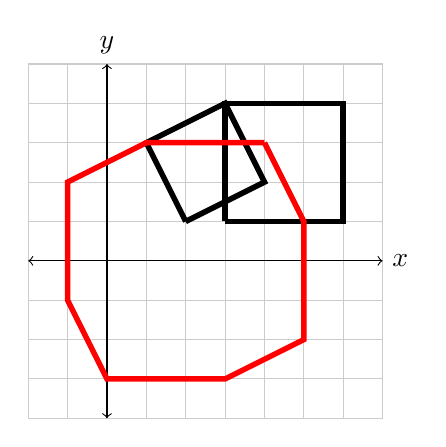
\begin{tikzpicture}[scale=0.5]
        \draw[thin,gray!40] (-2,-4) grid (7,5);
        \draw[<->] (-2,0)--(7,0) node[right]{$x$};
        \draw[<->] (0,-4)--(0,5) node[above]{$y$};
        \draw[line width=2pt,black](2,1) -- (1,3)--(3,4)--(4,2)--(2,1);
        \draw[line width=2pt,black](3,1) -- (3,4)--(6,4)--(6,1)--(3,1);
        \draw[line width=2pt,red](4,3)--(5,1)--(5,-2)--(3,-3)--(0,-3)--(-1,-1)--(-1,2)--(1,3)--(4,3);
    \end{tikzpicture}
    \caption{The Minkowski Difference hull. There are 16 total points we can calculate by finding the difference between each and every vertex, but only 8 of the resulting points act as vertices and form the hull, as all others fall somewhere within the hull}
    \label{fig:my_label}
\end{figure}
Then, we simply need to find if this hull contains the origin within it. GJK does this by working with something called a simplex, which is the bare minimum polytope that encloses a given point in $\mathbb{R}^n$. So for $\mathbb{R}^2$ this would be a triangle, as it is the bare minimum shape to enclose a point in 2 dimensions. If we are planning to implement this in 3 dimensions, our simplex is a tetrahedron. GJK works by finding a simplex bounded within the hull and doing a check if we contain the origin. If we do, we have collided and can move on. If we do not contain the origin, it finds the closest edge of the simplex to the origin, and generates a new simplex with that edge using points in the direction of the origin from that edge, as to progressively move towards the origin. If we do not contain the origin, and all the points in the direction of the origin are ones we have already used, then we know there is no such simplex bounded within our hull that will contain the origin, and thus we have not collided.
\\
\begin{figure}[!h]
    \centering
    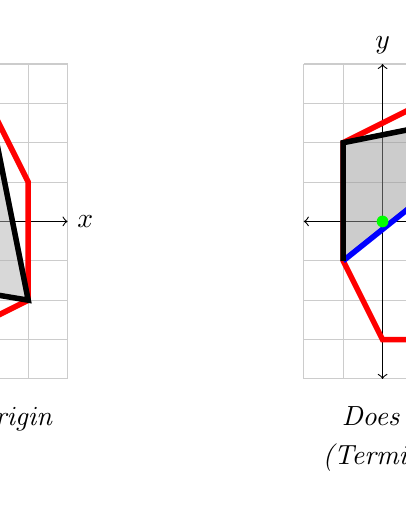
\begin{tikzpicture}[scale=0.5]
    \hspace{-3.5cm}
        \draw[thin,gray!40] (-2,-4) grid (6,4);
        \draw[<->] (-2,0)--(6,0) node[right]{$x$};
        \draw[<->] (0,-4)--(0,4) node[above]{$y$};
        \fill[black!30,semitransparent](4,3)--(5,-2)--(-1,-1)--(4,3);
        \draw[line width=2pt,red](4,3)--(5,1)--(5,-2)--(3,-3)--(0,-3)--(-1,-1)--(-1,2)--(1,3)--(4,3);
        \draw[line width=2pt,black](4,3)--(5,-2)--(-1,-1);
        \draw[line width=2pt,blue](-1,-1)--(4,3);
        \node at (0,0)[circle,fill,green,inner sep =1.5pt]{};
        \node at (2,-5) {\textit{Does not contain origin}};
        \hspace{7cm}
        \draw[thin,gray!40] (-2,-4) grid (6,4);
        \draw[<->] (-2,0)--(6,0) node[right]{$x$};
        \draw[<->] (0,-4)--(0,4) node[above]{$y$};
        \fill[black!40,semitransparent](4,3)--(-1,2)--(-1,-1)--(4,3);
        \draw[line width=2pt,red](4,3)--(5,1)--(5,-2)--(3,-3)--(0,-3)--(-1,-1)--(-1,2)--(1,3)--(4,3);
        \draw[line width=2pt,blue](-1,-1)--(4,3);
        \draw[line width=2pt,black](-1,-1)--(-1,2)--(4,3);
        \node at (0,0)[circle,fill,green,inner sep =1.5pt]{};
        \node at (2,-5) {\textit{Does contain origin}};
        \node at (2, -6) {\textit{(Termination Simplex)}};
    \end{tikzpicture}
    \caption{A simplex, with the closest edge to the origin coloured blue. The first simplex does not contain the origin, so we use this edge, and form another simplex using points in the direction of the origin from the closest edge}
\end{figure}
\section{EPA Also In A Nutshell}
Now, we need more information than just a simple yes or no answer to if we have collided. The Expanding Polytope Algorithm, or EPA, does just this. We take the termination simplex from GJK, and expand it using points from the Minkowski Difference hull. In particular, we want to find the edge of the polytope this forms that is closest to the origin. We can do this by looking only at the points on the hull in the direction of the normal of the closest edge on the termination simplex to the origin. This is because the termination simplex is generated by moving closer towards the origin in hopes to enclose it, and so the termination simplex should be in the region of the hull that has the origin closest to its edges. Once we have determined which edge of the expanded polytope is in fact the closest of all the possible edges from the original hull, we can use this edge and the origin to determine penetration depth and the normal of collision.  The normal of collision is the normal of the closest edge on our hull to the origin, and the depth of penetration is the distance between the origin and this edge. Thus, we can obtain our information about the collision normal and depth.
\begin{figure}[!ht]
    \centering
    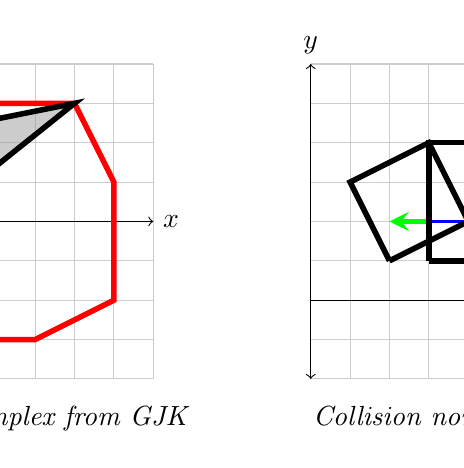
\begin{tikzpicture}[scale=0.5]
    \hspace{-3cm}
        \draw[thin,gray!40] (-2,-4) grid (6,4);
        \draw[<->] (-2,0)--(6,0) node[right]{$x$};
        \draw[<->] (0,-4)--(0,4) node[above]{$y$};
        \fill[black!40,semitransparent](4,3)--(-1,2)--(-1,-1)--(4,3);
        \draw[line width=2pt,red](4,3)--(5,1)--(5,-2)--(3,-3)--(0,-3)--(-1,-1)--(-1,2)--(1,3)--(4,3);
        \draw[line width=2pt,blue](-1,-1)--(-1,2);
        \draw[line width=2pt,black](-1,2)--(4,3)--(-1,-1);
        \draw[line width = 2pt, green,-stealth](0,0)--(-1,0);
        \node at (2,-5) {\textit{Termination Simplex from GJK}};
        \hspace{6cm}
        \draw[thin,gray!40] (-2,-4) grid (6,4);
        \draw[line width=2pt, green,-stealth](1,0)--(0,0);
        \draw[line width = 1pt, blue](1,0)--(2,0);
        \draw[->] (-2,-2)--(6,-2) node[right]{$x$};
        \draw[<->] (-2,-4)--(-2,4) node[above]{$y$};
        \draw[line width=2pt,black](0,-1) -- (-1,1)--(1,2)--(2,0)--(0,-1);
        \draw[line width=2pt,black](1,-1) -- (1,2)--(4,2)--(4,-1)--(1,-1);
        \node at (2,-5) {\textit{Collision normal \& depth}};
    \end{tikzpicture}
    \caption{The closest edge of the hull to the origin is used for the collision normal and depth. The length of the green vector on the left is the depth of collision, and its direction gives the normal. On the right, the blue line shows the depth is indeed 1, and the green vector showing the normal does indeed point orthogonally to the surface}
\end{figure}

\section{Bounded Volume Hierarchies}
So now that we know how to tell if we have collided, how do we figure out what object we actually want to check against? We could simply check against every solid object that exists, however, we would prefer to not have our game run like molasses. Doing GJK-EPA is kind of expensive to do, and so the less we have to do it, the better. If we have 10,000 objects in our world, we do not want to do this computation 10,000 times. Thus, we have the Bounded Volume Hierarchy (BVH). This is a structure that organizes our world in a way that vastly reduces the time taken to figure out what we collide with. Essentially, the world is first split into two (or some small number of) gigantic volumes that both enclose everything. Then, inside each volume, we split the remaining space into smaller volumes, and we continue to divide up the space until the smallest space contains our desired number of objects. When we go to check what we collide with, we will collide with one of the two largest boxes. From here, we can immediately eliminate half of the objects in the scene from needing a check. Then we check again with the sub-boxes, and eliminate half of the remaining objects, and we repeat checks until we have found the box containing the singular or few objects we wish to check directly against. Instead of needing to search $n$ times, once per object that exists in your scene (which will run in $\mathcal{O}(n)$ time), our search runs in $\mathcal{O}(\log(n))$, which is a considerable improvement.

\section{Binary Space Partitions}
Binary Space Partitions (BSP) is like BVH in that is also an acceleration structure, but it mainly plays important roles in figuring out what areas of the map are visible to the player in given areas, which is used to figure out what we want to render at any given time without the need for real-time computations (as a table of what should be rendered is stored in memory, and generated with the compiling of the map). However, many games (such as Quake and games that run on the Source engine) use BSP for collision detection as well.
\begin{figure}[H]
    \centering
    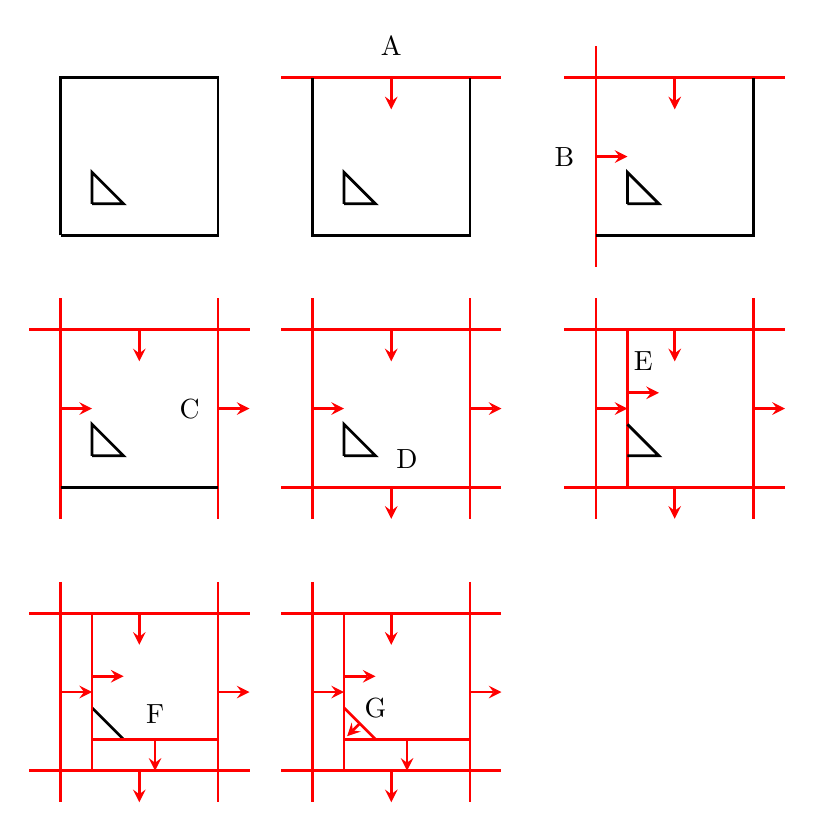
\begin{tikzpicture}[scale=0.4]
    % first
        \draw[line width=1pt,white](-1,0)--(6,0);
        \draw[line width=1pt,black](0,0)--(0,5)--(5,5)--(5,0)--(0,0);
        \draw[line width=1pt,black](1,1)--(1,2)--(2,1)--(1,1);
    % second
        \draw[line width=1pt,red](7,5)--(14,5);
        \draw[line width=1pt,red,-stealth](10.5,5)--(10.5,4);
        \draw[line width=1pt,black](8,5)--(8,0)--(13,0)--(13,5);
        \draw[line width=1pt,black](9,1)--(10,1)--(9,2)--(9,1);

        \node at (10.5,6){A};
    % third
        \draw[line width=1pt,red](16,5)--(23,5);
        \draw[line width=1pt,red,-stealth](17,2.5)--(18,2.5);
        \draw[line width=1pt,red](17,6)--(17,-1);
        \draw[line width=1pt,red,-stealth](19.5,5)--(19.5,4);
        \draw[line width=1pt,black](17,0)--(22,0)--(22,5);
        \draw[line width=1pt,black](18,1)--(18,2)--(19,1)--(18,1);

        \node at (16,2.5){B};
    % fourth
        \draw[line width=1pt,red](0,-2)--(0,-9);
        \draw[line width=1pt,red,-stealth](0,-5.5)--(1,-5.5);
        \draw[line width=1pt,red](-1,-3)--(6,-3);
        \draw[line width=1pt,red,-stealth](2.5,-3)--(2.5,-4);
        \draw[line width=1pt,red](5,-2)--(5,-9);
        \draw[line width=1pt,red,-stealth](5,-5.5)--(6,-5.5);
        \draw[line width=1pt,black](0,-8)--(5,-8);
        \draw[line width=1pt,black](1,-7)--(2,-7)--(1,-6)--(1,-7);

        \node at (4.1,-5.5){C};
    % fifth
        \draw[line width=1pt,red](7,-3)--(14,-3);
        \draw[line width=1pt,red,-stealth](10.5,-3)--(10.5,-4);
        \draw[line width=1pt,red](8,-2)--(8,-9);
        \draw[line width=1pt,red,-stealth](8,-5.5)--(9,-5.5);
        \draw[line width=1pt,red](7,-8)--(14,-8);
        \draw[line width=1pt,red,-stealth](10.5,-8)--(10.5,-9);
        \draw[line width=1pt,red](13,-9)--(13,-2);
        \draw[line width=1pt,red,-stealth](13,-5.5)--(14,-5.5);
        \draw[line width=1pt,black](9,-7)--(9,-6)--(10,-7)--(9,-7);

        \node at (11,-7.1){D};
    % sixth
        \draw[line width=1pt,red](16,-3)--(23,-3);
        \draw[line width=1pt,red,-stealth](19.5,-3)--(19.5,-4);
        \draw[line width=1pt,red](17,-2)--(17,-9);
        \draw[line width=1pt,red,-stealth](17,-5.5)--(18,-5.5);
        \draw[line width=1pt,red](16,-8)--(23,-8);
        \draw[line width=1pt,red,-stealth](19.5,-8)--(19.5,-9);
        \draw[line width=1pt,red](22,-9)--(22,-2);
        \draw[line width=1pt,red,-stealth](22,-5.5)--(23,-5.5);
        \draw[line width=1pt,red](18,-3)--(18,-8);
        \draw[line width=1pt,red,-stealth](18,-5)--(19,-5);
        \draw[line width=1pt,black](18,-7)--(19,-7)--(18,-6);

        \node at (18.5,-4){E};
    % seventh
        \draw[line width=1pt,red](-1,-12)--(6,-12);
        \draw[line width=1pt,red,-stealth](2.5,-12)--(2.5,-13);
        \draw[line width=1pt,black](1,-15)--(2,-16);
        \draw[line width=1pt,red](0,-11)--(0,-18);
        \draw[line width=1pt,red,-stealth](0,-14.5)--(1,-14.5);
        \draw[line width=1pt,red](-1,-17)--(6,-17);
        \draw[line width=1pt,red,-stealth](2.5,-17)--(2.5,-18);
        \draw[line width=1pt,red](5,-11)--(5,-18);
        \draw[line width=1pt,red,-stealth](5,-14.5)--(6,-14.5);
        \draw[line width=1pt,red](1,-12)--(1,-17);
        \draw[line width=1pt,red,-stealth](1,-14)--(2,-14);
        \draw[line width=1pt,red](1,-16)--(5,-16);
        \draw[line width=1pt,red,-stealth](3,-16)--(3,-17);

        \node at (3,-15.2){F};
    % eigth
        %top line
        \draw[line width=1pt,red](7,-12)--(14,-12);
        \draw[line width=1pt,red,-stealth](10.5,-12)--(10.5,-13);
        % angle
        \draw[line width=1pt,red](9,-15)--(10,-16);
        \draw[line width=1pt,red,-stealth](9.5,-15.5)--(9.1,-15.9);

        \node at (10,-15){G};
        % inner left line
        \draw[line width=1pt,red](9,-12)--(9,-17);
        \draw[line width=1pt,red,-stealth](9,-14)--(10,-14);
        % bottom line
        \draw[line width=1pt,red](7,-17)--(14,-17);
        \draw[line width=1pt,red,-stealth](10.5,-17)--(10.5,-18);
        % right line
        \draw[line width=1pt,red](13,-11)--(13,-18);
        \draw[line width=1pt,red,-stealth](13,-14.5)--(14,-14.5);
        % left line
        \draw[line width=1pt,red](8,-11)--(8,-18);
        \draw[line width=1pt,red,-stealth](8,-14.5)--(9,-14.5);
        % inner bottom line
        \draw[line width=1pt,red](9,-16)--(13,-16);
        \draw[line width=1pt,red,-stealth](11,-16)--(11,-17);
        
        \end{tikzpicture}
        \caption{Example BSP partitioning}
\end{figure}
The basic premise is that we recursively slice up our map along each face, and store it in a particular manner to accelerate such searches for collisions and rendering. A binary tree is then organized with the first face at the top. Anything on one side of the slice along the face is then put onto one side of the tree, and everything else is put onto the other side. We recursively slice each face in each leaf, and continue to separate the remaining portions of the world based on what falls on either side of the slice. \\
\\
Once we have a full tree, we can make use of this for rendering purposes very easily. If we know our player sits on one side of a plane, we can immediately eliminate the leaf on the opposite side of the tree to where we are, which thereby eliminates all subsequent branches of the tree on that side. Each time we determine which side of a plane we are on we can drastically reduce the number of remaining planes to consider rendering, and efficiently build a table of which planes to render when in certain areas. A similar process can be used for collision purposes, although rendering was the main motivation for the implementation of this structure.

\section{The Collision Hull}
In Quake and subsequent games based on the Source engine, the player interacts with the world physically by means of an Axis-Aligned Bounding Box (AABB). An AABB is a box that remains aligned no matter what, so rotating the players view by looking around does not change the rotation of this box. This is often referred to as the collision hull, as it is used to calculate collisions (and also splash damage). Quake handles collisions via something called $\texttt{pmtrace\_t}$. A trace essentially continuously moves a collision hull sized box along a path, and collects information about any solids it collides with along the way. It returns a fraction between 0 and 1, which represents the portion of its path that it was able to travel before collision. For example, if this fraction is 1, then it travelled all the way without colliding. If this fraction was 0.5, then it would have travelled half of its distance before colliding, and so on. It also returns the normal vectors for the planes it collided with. We can use GJK-EPA or some algorithm similar to it to determine this information. Thus, on each frame we can give the trace our current position as a starting point, and move it from our position to the position we intend to end up with our current velocity. This way, the trace will tell us the maximum step forward we can make in this direction that does not put us inside of a solid (using the trace fraction). As well, we want to remove the component of our velocity in the direction of the normals of collision. Explicitly, for a normal $\vec{n}$ and player velocity $\vec{v}$, we can edit our velocity to move parallel with $\vec{v} - (\vec{v}\cdot\vec{n})\vec{n}$. Thus, our velocity puts us along the surface, so we slide along it instead of entirely coming to a halt when impacting a surface. There is much more nuance to this, but most of it will be explained later during the discussion of the actual movement functions that Quake uses. 
\newpage
\part{So Now We Can Actually Move, I Guess}
\section{PM\_ClipVelocity}
To begin working with collision detection, we need something that takes care of properly projecting our velocities along the planes we will collide with. For the unfamiliar, vector projection gives you the component/portion of one vector in the direction of another vector. One other important thing to note about this is that if two vectors have a $90^{\circ}$ to each other, then they share no component in the direction of each other. We give this the special name of being 'orthogonal', as sometimes angles between vectors does not really make sense, but the notion of orthogonality remains useful, thus this abstracted term is nice to have.
\begin{minted}[linenos,tabsize=2,breaklines,firstnumber=72]{c}
int PM_ClipVelocity (vec3_t in, vec3_t normal, vec3_t out, float overbounce)
{
	float	backoff;
	float	change;
	int		i, blocked;
	
	blocked = 0;
	if (normal[2] > 0)
		blocked |= 1;		// floor
	if (!normal[2])
		blocked |= 2;		// step
	
	backoff = DotProduct (in, normal) * overbounce;

	for (i=0 ; i<3 ; i++)
	{
		change = normal[i]*backoff;
		out[i] = in[i] - change;
		if (out[i] > -STOP_EPSILON && out[i] < STOP_EPSILON)
			out[i] = 0;
	}
	
	return blocked;
}
\end{minted}
This function is passed a vector we want to project along a surface, the surface normal, the vector to copy the result into, and a float called $\texttt{overbounce}$ which acts as yet another epsilon value. First, we determine if the normal is a floor, which is if it has a $z$-component greater than 0, or if the surface normal is for a wall which would  be a $z$-component of 0. Next, we find the component of our velocity in the direction of the normal, scaled a bit extra by the variable $\texttt{overbounce}$, and we subtract this from our input vector. If we have an $\texttt{overbounce}$ value >1, then some portion of our velocity points back towards us, and thus we do not actually move parallel to the plane. Lastly, if any of the components of the output vector are within the bounds of $\lvert \texttt{STOP\_EPSILON} \rvert$, we set the component to 0. This prevents us from having extremely small movements when against planes, and lets us snap to a stop when we collide with sufficiently slow speeds. The result is already stored in the vector $\texttt{out}$, and so we return the $\texttt{blocked}$ flag. Interesting to note that this return value is never used, and later in Quake 3 this becomes a void function. 
\section{PM\_FlyMove}
We actually want to implement a more general movement function first. $\texttt{PM\_FlyMove}$ handles translating the player in all 3 dimensions, and later the function $\texttt{PM\_GroundMove}$ handles moving when on the ground in particular. This is because we want to include specific extra math for handling stairs and such, and thus separating the general collision detection and movement into one function allows us to just call this function when we may need it in the more specific function later on. Thus, understanding $\texttt{PM\_FlyMove}$ is important for movement here on out. Let us take a look at how it is written:
\begin{minted}[linenos,tabsize=2,breaklines,firstnumber=128]{c}
	time_left = frametime;

	for (bumpcount=0 ; bumpcount<numbumps ; bumpcount++)
	{
		for (i=0 ; i<3 ; i++)
			end[i] = pmove.origin[i] + time_left * pmove.velocity[i];

		trace = PM_PlayerMove (pmove.origin, end);

		if (trace.startsolid || trace.allsolid)
		{	// entity is trapped in another solid
			VectorCopy (vec3_origin, pmove.velocity);
			return 3;
		}

		if (trace.fraction > 0)
		{	// actually covered some distance
			VectorCopy (trace.endpos, pmove.origin);
			numplanes = 0;
		}

		if (trace.fraction == 1)
			 break;		// moved the entire distance
\end{minted}

This mainly does what we described the collision hull to do in the section above. It manually compiles a list of every plane it intersects with and does a variety of tricks to determine how we should move. 

\begin{minted}[linenos,tabsize=2,breaklines,firstnumber=137]{c}
if (trace.startsolid || trace.allsolid)
		{	// entity is trapped in another solid
			VectorCopy (vec3_origin, pmove.velocity);
			return 3;
		}

		if (trace.fraction > 0)
		{	// actually covered some distance
			VectorCopy (trace.endpos, pmove.origin);
			numplanes = 0;
		}
  
		if (trace.fraction == 1)
			 break;		// moved the entire distance
\end{minted}
The first of these checks is a basic check to determine if our trace begins already inside an object, in which case we are probably stuck inside an object. The next check takes a look at the trace fraction. If it is greater than 0, then we know we covered some distance without colliding, and so we should move some amount based on this fraction (which we will do later). If it is 1, then we have moved the entire distance without colliding, and so we do not have to worry about editing our path.
\begin{minted}[linenos,tabsize=2,breaklines,firstnumber=156]{c}
if (trace.plane.normal[2] > 0.7)
		{
			blocked |= 1;		// floor
		}
		if (!trace.plane.normal[2])
		{
			blocked |= 2;		// step
		}
\end{minted}
The next check that Quake makes is in relation to sloped surfaces. We want to move along surfaces that do not slope very much as though we were on normal ground, and we want to slide down surfaces with sufficiently high slopes.  This very simple check does not need to compute any angles or dot products to determine the slope, but instead references a nice observation: any normalized vector that has a component in the $z$ direction greater than 0.7 will have a slope less than $45^{\circ}$. This is because if we consider a unit vector that points directly upward, and begin to rotate it towards the $xy$-plane, it will progressively decrease in its $z$-component. The magic number for a slope of roughly $45^{\circ}$ is when it has a component of 0.7 in the $z$-axis. Any less, and the normal of collision points at a shallow angle from the $xy$-plane, which means the actual surface is at a larger angle. The second check is to make sure we even have a $z$-component. If we do not, then we know the surface normal must be perfectly at $90^{\circ}$ to the $xy$-plane, meaning we are colliding with a flat wall and not a slope of some sort. In this case, we would want to additionally run a check to see if we can step up a stair height and move forward, as we do not want to simply slam into a 1-unit tall piece of geometry and stop moving. If it was slanted we would move up it, if it is a wall it has the potential to be a step. 
\begin{minted}[linenos,tabsize=2,breaklines,firstnumber=165]{c}
time_left -= time_left * trace.fraction;
		
	// cliped to another plane
		if (numplanes >= MAX_CLIP_PLANES)
		{	// this shouldn't really happen
			VectorCopy (vec3_origin, pmove.velocity);
			break;
		}
\end{minted}
The first line here finds the time we spent travelling before collision, and subtracts that from the total time we have between frames, leaving us with the amount of time that we would spend moving inside the object we collide with. Next, we do a quick check to see if we collide with more planes than the cvar $\texttt{MAX\_CLIP\_PLANES}$, which by default is 4. If we collide with more than 4 planes, we do not do anything.
\begin{minted}[linenos,tabsize=2,breaklines,firstnumber=178]{c}
// modify original_velocity so it parallels all of the clip planes
//
		for (i=0 ; i<numplanes ; i++)
		{
			PM_ClipVelocity (original_velocity, planes[i], pmove.velocity, 1);
			for (j=0 ; j<numplanes ; j++)
				if (j != i)
				{
					if (DotProduct (pmove.velocity, planes[j]) < 0)
						break;	// not ok
				}
			if (j == numplanes)
				break;
		}
		
		if (i != numplanes)
		{	// go along this plane
		}
		else
		{	// go along the crease
			if (numplanes != 2)
			{
//				Con_Printf ("clip velocity, numplanes == %i\n",numplanes);
				VectorCopy (vec3_origin, pmove.velocity);
				break;
			}
			CrossProduct (planes[0], planes[1], dir);
			d = DotProduct (dir, pmove.velocity);
			VectorScale (dir, d, pmove.velocity);
		}
\end{minted}
Now that we have determined generally what it is that we have collided with, such as a wall or ramp, we can move accordingly. For each plane that we intersect, we want to project our velocity along the plane using its normal. This is where we use $\texttt{PM\_ClipVelocity}$. As well, we consider the dot product of this adjusted velocity against the normal of the other planes we collide with. If this dot product is positive, then we have some component of our velocity in the same direction as the normal, meaning we are moving into the plane. We do not want to do this, so we break. Otherwise, we want to do a check to see if we collide with 1 or more planes. If we collide with 1 plane, we just move along it. If we collide with 2, we take the cross product of the two planes we collide with, and project our velocity onto the cross product.
This may seem odd, but it makes sense if we consider a few examples:
\begin{figure}[H]
    \centering
    \tdplotsetmaincoords{70}{135}
    \begin{tikzpicture}[scale=0.5,tdplot_main_coords,grid/.style={very thin,gray}]
        \hspace{-2.5cm}
            \fill[gray!40, semitransparent](0,0,0)--(5,0,0)--(5,5,0)--(0,5,0)--(0,0,0);
            % grid, y
            \draw[line width=1pt,gray](5,0,0)--(5,5,0);
            \draw[line width=1pt,gray](4,0,0)--(4,5,0);
            \draw[line width=1pt,gray](3,0,0)--(3,5,0);
            \draw[line width=1pt,gray](2,0,0)--(2,5,0);
            \draw[line width=1pt,gray](1,0,0)--(1,5,0);

            \draw[line width=1pt,gray](0,5,0)--(5,5,0);
            \draw[line width=1pt,gray](0,4,0)--(5,4,0);
            \draw[line width=1pt,gray](0,3,0)--(5,3,0);
            \draw[line width=1pt,gray](0,2,0)--(5,2,0);
            \draw[line width=1pt,gray](0,1,0)--(5,1,0);

            \draw[line width=1pt,-stealth](0,0,0)--(5,0,0);
            \node at (5.5,0,0){\textit{$\vec{a}$}};
            \draw[line width=1pt,-stealth](0,0,0)--(0,5,0);
            \node at (0,5.5,0){\textit{$\vec{b}$}};
            \draw[line width=1pt,red,-stealth](0,0,0)--(0,0,5);
            \node at (0,0,5.5){\textit{$\vec{a}\times\vec{b}$}
            };
        \hspace{5cm}
    % (x,y,z) as in fig 8
    % GRID
        % front left
        \draw[line width=0.5pt,gray](3,-3,0)--(3,3,0);
        % front right
        \draw[line width=0.5pt,gray](-3,3,0)--(3,3,0);
        % back right
        \draw[line width=0.5pt,gray](-3,0,0)--(-3,3,0);
        % back left
        \draw[line width=0.5pt,gray](0,-3,0)--(3,-3,0);
        % inner right
        \draw[line width=0.5pt,gray](0,1.5,0)--(3,1.5,0);
        % inner left
        \draw[line width=0.5pt,gray](1.5,0,0)--(1.5,3,0);
        % back inner left
        \draw[line width=0.5pt,gray](1.5,-3,0)--(1.5,-1.5,0);
        % back inner right
        \draw[line width=0.5pt,gray](-3,1.5,0)--(-1.5,1.5,0);
        % back angled down left
        \draw[line width=0.5pt,gray](3,-1.5,0)--(1.5,-1.5,0);
        \draw[line width=0.5pt,gray](-1.5,3,0)--(-1.5,1.5,0);
    % PLANES
        \draw[line width=1pt](0,0,0)--(0,0,3)--(3,0,3)--(3,0,0)--(0,0,0);
        \draw[line width=1pt](0,0,0)--(0,3,0)--(0,3,3)--(0,0,3);
    % AXES
        \draw[line width=1pt,-stealth](0,0,0)--(5,0,0);
        \node at (5.5,0,0){\textit{x}};
        \draw[line width=1pt,-stealth](0,0,0)--(0,5,0);
        \node at (0,5.5,0){\textit{y}};
        \draw[line width=1pt,red,-stealth](0,0,0)--(0,0,5);
        \node at (0,0,5.5){\textit{z}
        };
    % normals
        \draw[line width=1pt,-stealth](1.5,0,1.5)--(1.5,1,1.5);
        \draw[line width=1pt,-stealth](0,1.5,1.5)--(1,1.5,1.5);
    \end{tikzpicture}
    \caption{Left: The cross product of a vector $\vec{a}$ with a vector $\vec{b}$, denoted in red. The length of the cross product is the area of the shaded area. Right: An example of two planes forming a corner. The planes normals are shown, and the cross product points straight up along the $z$-axis}
    \end{figure}
If we collide with two walls at once, we are in a corner and thus do not want to move horizontally. The cross product of two normals that point straight out towards us must give a vector that points directly up or down, meaning that unless we are falling or jumping, any horizontal components of our velocity will be nuked in the projection onto the cross product, giving us a velocity of 0 as we intend. \\
\\
If we also consider sloped surfaces, it makes sense. Consider falling into a V-shaped wedge between two ramps. The cross product of the two normals would produce a vector that points along the crease, meaning our velocity moves us along the surface of the two ramps, as we'd expect. 
\begin{minted}[linenos,tabsize=2,breaklines,firstnumber=210]{c}
// if original velocity is against the original velocity, stop dead
// to avoid tiny occilations in sloping corners
//
		if (DotProduct (pmove.velocity, primal_velocity) <= 0)
		{
			VectorCopy (vec3_origin, pmove.velocity);
			break;
		}
	}

	if (pmove.waterjumptime)
	{
		VectorCopy (primal_velocity, pmove.velocity);
	}
	return blocked;
}
\end{minted}
The last portion of $\texttt{PM\_FlyMove}$ takes care of the case when our updated velocity points orthogonal or backwards to the original velocity, and if so, we halt. This ensures we do not get stuck in a weird cycle of moving some super small amount towards a wall, getting moved back a bit, and then able to move forwards that bit again, and repeatedly oscillating between hitting a wall and being pushed back. 
\section{PM\_GroundMove}
This function takes care of more of the specific motion when on the ground, such as stairs. Some of it may seem familiar: 
\begin{minted}[linenos,tabsize=2,breaklines,firstnumber=241]{c}
	pmove.velocity[2] = 0;
	if (!pmove.velocity[0] && !pmove.velocity[1] && !pmove.velocity[2])
		return;

	// first try just moving to the destination	
	dest[0] = pmove.origin[0] + pmove.velocity[0]*frametime;
	dest[1] = pmove.origin[1] + pmove.velocity[1]*frametime;	
	dest[2] = pmove.origin[2];

	// first try moving directly to the next spot
	VectorCopy (dest, start);
	trace = PM_PlayerMove (pmove.origin, dest);
	if (trace.fraction == 1)
	{
		VectorCopy (trace.endpos, pmove.origin);
		return;
	}
\end{minted}
First, we set the $z$-component of our velocity to 0, and then check if we have a non-zero velocity in the $xy$-plane. If we are moving extremely slow, we do not need to move at all, and so we return. Otherwise, we continue with setting the vector $\texttt{dest}$ to be where we will end up with our current velocity after the current frame. If our trace does not hit anything from our position to destination we can move the whole distance, and so we set our origin to the destination. 
\begin{minted}[linenos,tabsize=2,breaklines,firstnumber=259]{c}
// try sliding forward both on ground and up 16 pixels
	// take the move that goes farthest
	VectorCopy (pmove.origin, original);
	VectorCopy (pmove.velocity, originalvel);

	// slide move
	PM_FlyMove ();

	VectorCopy (pmove.origin, down);
	VectorCopy (pmove.velocity, downvel);

	VectorCopy (original, pmove.origin);
	VectorCopy (originalvel, pmove.velocity);
\end{minted}
First, it should be noted that the comment here references the piece of code \textit{following} this block of code, which is the height for if we can step up a stair height and move forward. For now, this block of code simply uses the pre-existing $\texttt{PM\_FlyMove}$ to take care of collisions that we encounter, which is mainly making sure we project our velocity properly with everything we collide with. Then, we just store the step that this takes. Then, we check stair height motion:
\begin{minted}[linenos,tabsize=2,breaklines,firstnumber=273]{c}
// move up a stair height
	VectorCopy (pmove.origin, dest);
	dest[2] += STEPSIZE;
	trace = PM_PlayerMove (pmove.origin, dest);
	if (!trace.startsolid && !trace.allsolid)
	{
		VectorCopy (trace.endpos, pmove.origin);
	}

// slide move
	PM_FlyMove ();

// press down the stepheight
	VectorCopy (pmove.origin, dest);
	dest[2] -= STEPSIZE;
	trace = PM_PlayerMove (pmove.origin, dest);
	if ( trace.plane.normal[2] < 0.7)
		goto usedown;
	if (!trace.startsolid && !trace.allsolid)
	{
		VectorCopy (trace.endpos, pmove.origin);
	}
	VectorCopy (pmove.origin, up);
\end{minted}
This adds a stair height to our stored destination, and attempts to move us from our position to our destination offset vertically by a stair height. This takes care of moving horizontally into the stairs. Now that we end up somewhere either directly on the stair or slightly above it, we want to move our player downwards to rest on top of the stairs. Thus, we once more do a trace down to determine how far down we have to go until we land on the step. If we land on a valid ground surface, we skip ahead to later in the code. Otherwise, so long as we do not start or end inside a solid, we move to our new destination with the vertical offset included. 
\begin{minted}[linenos,tabsize=2,breaklines,firstnumber=297]{c}
// decide which one went farther
	downdist = (down[0] - original[0])*(down[0] - original[0])
		+ (down[1] - original[1])*(down[1] - original[1]);
	updist = (up[0] - original[0])*(up[0] - original[0])
		+ (up[1] - original[1])*(up[1] - original[1]);

	if (downdist > updist)
	{
usedown:
		VectorCopy (down, pmove.origin);
		VectorCopy (downvel, pmove.velocity);
	} else // copy z value from slide move
		pmove.velocity[2] = downvel[2];
\end{minted}
This does exactly as commented. It checks if we went further using $\texttt{PM\_FlyMove}$ or the stair height additional move, and we use whichever made us move further. After this, there is an additional comment relating to nudging the player, however there actually is not any code after this point.
\section{PM\_CatagorizePosition}
The last check we have to do in our movement is a more complex check for if we are grounded or not, to be able to determine what functions to use when moving. This is the job of $\texttt{PM\_CatagorizePosition}$, and yes they did spell Categorize incorrectly. There are many spelling errors in the code's comments as well, which is quite funny. Below is the implementation:
\begin{minted}[linenos,tabsize=2,breaklines,firstnumber=580]{c}
// if the player hull point one unit down is solid, the player
// is on ground

// see if standing on something solid	
	point[0] = pmove.origin[0];
	point[1] = pmove.origin[1];
	point[2] = pmove.origin[2] - 1;
	if (pmove.velocity[2] > 180)
	{
		onground = -1;
	}
	else
	{
		tr = PM_PlayerMove (pmove.origin, point);
		if ( tr.plane.normal[2] < 0.7)
			onground = -1;	// too steep
		else
			onground = tr.ent;
		if (onground != -1)
		{
			pmove.waterjumptime = 0;
			if (!tr.startsolid && !tr.allsolid)
				VectorCopy (tr.endpos, pmove.origin);
		}

		// standing on an entity other than the world
		if (tr.ent > 0)
		{
			pmove.touchindex[pmove.numtouch] = tr.ent;
			pmove.numtouch++;
		}
	}
\end{minted}
Essentially, we first store our position into the vector $\texttt{point}$, and subtract 1 unit from our height, which will be used as a sort of destination for our trace to use so we can check for planes below us. If we have an upward component in our velocity that exceeds 180 units per second, then we are considered airborne. This has the consequences of allowing us to slide up ramps that are less than $45^{\circ}$ from the ground (the ramps we would normally just walk up). When we hit the ramp, and our velocity is projected along the ramp, some of our horizontal velocity is given to our vertical component during the projection, and provided our velocity is large enough, we can achieve an upwards component of greater than 180 units per second. \\
\\
Next, we check if we collide with anything 1 unit below us. If we do, we check if it is too steep. If it is sloped less than $45^{\circ}$, then we consider ourselves grounded. Otherwise, we are airborne. Lastly, if we are found to be standing on an entity, we record what entity we are standing on, as this is used to trigger some events such as waking up enemies if we stand on their head.
\section{NudgePosition}
This function serves the purpose of quite literally nudging the player out of a solid object if they are stuck in it. It utilizes a function $\texttt{PM\_TestPlayerPosition}$ which essentially just checks if the collision hull intersects some other entity in the world such as world geometry. Such a function is built on a fair amount of helper functions that do a lot of very funny math and if I opted to include it all here to explain precisely how it works this paper would be twice as long. It suffices for our purposes to know that all of this just checks if we intersect something. With that in mind, here is the implementation for nudging players out of solids:
\begin{minted}[linenos,tabsize=2,breaklines,firstnumber=742]{c}
	VectorCopy (pmove.origin, base);

	for (i=0 ; i<3 ; i++)
		pmove.origin[i] = ((int)(pmove.origin[i]*8)) * 0.125;
//	pmove.origin[2] += 0.124;

//	if (pmove.dead)
//		return;		// might be a squished point, so don'y bother
//	if (PM_TestPlayerPosition (pmove.origin) )
//		return;

	for (z=0 ; z<=2 ; z++)
	{
		for (x=0 ; x<=2 ; x++)
		{
			for (y=0 ; y<=2 ; y++)
			{
				pmove.origin[0] = base[0] + (sign[x] * 1.0/8);
				pmove.origin[1] = base[1] + (sign[y] * 1.0/8);
				pmove.origin[2] = base[2] + (sign[z] * 1.0/8);
				if (PM_TestPlayerPosition (pmove.origin))
					return;
			}
		}
	}
	VectorCopy (base, pmove.origin);
//	Con_DPrintf ("NudgePosition: stuck\n");
}
\end{minted}
After setting up some initial values for our tests, we essentially loop through each coordinate axis and try adding or subtracting some small delta value, approximately $\frac{1}{8}$ of a unit, until we can get a combination of nudges forward or backward on each axis that gives us a valid position. The values $x,y,z$ in the $\texttt{for}$ loops determine if the array $\texttt{sign}$ gives us 0, -1, or 1, which gives us either no nudge, a nudge by $\frac{1}{8}$-th of a unit forward, or backward on that axis. Thus we can achieve every possible combination of nudges with these nested $\texttt{for}$ loops.
\section{Tying It All Together: MovePlayer}
Now that we have all of the necessary functions to handle user input, velocity, acceleration, collisions, ground state, and more, we can finally tie them all together into one function that handles the order of execution of each and passes information between them. This is the $\texttt{MovePlayer}$ function:
\begin{minted}[linenos,tabsize=2,breaklines,firstnumber=862]{c}
void PlayerMove (void)
{
	frametime = pmove.cmd.msec * 0.001;
	pmove.numtouch = 0;

	AngleVectors (pmove.angles, forward, right, up);

	if (pmove.spectator)
	{
		SpectatorMove ();
		return;
	}

	NudgePosition ();

	// take angles directly from command
	VectorCopy (pmove.cmd.angles, pmove.angles);

	// set onground, watertype, and waterlevel
	PM_CatagorizePosition ();

	if (waterlevel == 2)
		CheckWaterJump ();

	if (pmove.velocity[2] < 0)
		pmove.waterjumptime = 0;

	if (pmove.cmd.buttons & BUTTON_JUMP)
		JumpButton ();
	else
		pmove.oldbuttons &= ~BUTTON_JUMP;

	PM_Friction ();

	if (waterlevel >= 2)
		PM_WaterMove ();
	else
		PM_AirMove ();

	// set onground, watertype, and waterlevel for final spot
	PM_CatagorizePosition ();
}
\end{minted}
We begin by orienting our space to be relative to our camera's perspective using the $\texttt{AngleVectors}$ function, which is discussed in the math function reference section. This just makes sure that user input remains relative to the direction we are looking in. Then, we check if we are dead or in spectator, to either not move (dead) or use the spectator movement function, which I have chosen to exclude (it is fairly straight forward movement without any collision checks). Next, we call $\texttt{NudgePosition}$ in case we managed to get stuck inside an object on the last frame. We then check our ground state, and consider if we can jump or not based on user input and ground state. I have chosen not to include the function $\texttt{JumpButton}$ as a majority of it is water-related, and the only significant portion of it simply adds 270 units per second upward to the player's velocity, and sets us to not be grounded. After this, we apply friction, and execute $\texttt{PM\_AirMove}$ to figure out our intended direction to move in. It is within this function that we determine if we should use the air or grounded acceleration and movement functions, and thus, we do not need to call it here. Finally, we determine if our new position is grounded or not via a call to $\texttt{PM\_CatagorizePosition}$. With all of this, we have successfully moved some distance over the course of 1 singular frame.
\section{Closing Remarks}
I have chosen to ignore several functions included in the $\texttt{pmove.c}$ file as the main purpose of this document is about normal movement. I have excluded water movement and spectator movement, and where there was a significant portion of code relating to these, I have elected to remove them for sake of clarity and page count. As well, I have chosen to excluded the $\texttt{JumpButton}$ function as well, as a huge majority of its code is in relation to water, and the main few lines were trivial.
\newpage
\part{Brief Reference for Math Functions Used}
\section{About This Section}
Throughout this code, we make extensive use of various helper math functions. I have decided to include their code, along with a brief description of what it does both mathematically and geometrically where applicable. These functions are written in the order they appear in the $\texttt{pmove.c}$ file, and all can be found within the $\texttt{mathlib.c}$ file in the same directory.
\section{DotProduct}
\begin{minted}[linenos,tabsize=2,breaklines,firstnumber=335]{c}
vec_t _DotProduct (vec3_t v1, vec3_t v2)
{
	return v1[0]*v2[0] + v1[1]*v2[1] + v1[2]*v2[2];
}

\end{minted}
Quite simply, this returns a scalar that is the sum of the component-wise multiplication of two vectors. Similarly, this can be calculated with $\parallel\vec{a}\parallel \parallel\vec{b}\parallel\cos{\theta}$, where $\vec{a},\vec{b}\in\mathbb{R}^2$ and $\theta$ is the angle between them. It is both faster and more general to higher dimension spaces or spaces with no general notion of angles to compute the inner product, which is essentially the same thing, but does not involve cosines or angles. This is $\sum_{i=1}^n a_i b_i$, where $\vec{a},\vec{b}\in\mathbb{R}^n$ and $n$ is the dimension of the space. This formula is what is explicitly written here. \\
\\
The notable properties of the dot product are that when the angle between them is $90^{\circ}$, the dot product is 0 (or more generally we say that the vectors are \textit{orthogonal}.) As well, if the two vectors point greater than $90^{\circ}$ from each other, the dot product is negative. We can then use this check of whether the result is negative, 0, or positive to determine a lot of key information about the direction between two vectors without ever needing to explicitly find angles. 
\section{VectorCopy}
\begin{minted}[linenos,tabsize=2,breaklines,firstnumber=354]{c}
void _VectorCopy (vec3_t in, vec3_t out)
{
	out[0] = in[0];
	out[1] = in[1];
	out[2] = in[2];
}
\end{minted}
This quite literally copies the contents of the vector $\texttt{in}$ into the vector $\texttt{out}$. Nothing much more to say.
\section{CrossProduct}
\begin{minted}[linenos,tabsize=2,breaklines,firstnumber=361]{c}
void CrossProduct (vec3_t v1, vec3_t v2, vec3_t cross)
{
	cross[0] = v1[1]*v2[2] - v1[2]*v2[1];
	cross[1] = v1[2]*v2[0] - v1[0]*v2[2];
	cross[2] = v1[0]*v2[1] - v1[1]*v2[0];
}
\end{minted}
This product can also be expressed with two different formulas. The one used here does not involve angles or sine, and is thus a lot nicer to compute. A slightly visually nicer way of seeing this computation is:
\begin{align*}
\begin{bmatrix}
c_1 \\
c_2 \\
c_3
\end{bmatrix}
 &= 
 \begin{bmatrix}
     a_2 b_3 - a_3 b_2 \\
     a_3 b_1 - a_1 b_3 \\
     a_1 b_2 - a_2 b_1
 \end{bmatrix}
\end{align*}
for some two input vectors $\vec{a},\vec{b}\in\mathbb{R}^n$, which yields a vector $\vec{c}\in\mathbb{R}^n$. Geometrically, this outputs a vector orthogonal to both input vectors, with a length equal to the area given by the parallelogram with both input vectors for sides. Thus, if they  point in the same direction or opposite, this area would be 0, and so the cross product  would be the zero vector. We only use this in $\texttt{PM\_FlyMove}$ to find a vector orthogonal to both planes we collide with.
\section{VectorScale}
\begin{minted}[linenos,tabsize=2,breaklines,firstnumber=409]{c}
void VectorScale (vec3_t in, vec_t scale, vec3_t out)
{
	out[0] = in[0]*scale;
	out[1] = in[1]*scale;
	out[2] = in[2]*scale;
}
\end{minted}
This simply takes in a vector and a scalar, and returns a vector that is the input scaled by the scalar.
\section{VectorNormalize}
\begin{minted}[linenos,tabsize=2,breaklines,firstnumber=383]{c}
float VectorNormalize (vec3_t v)
{
	float	length, ilength;

	length = v[0]*v[0] + v[1]*v[1] + v[2]*v[2];
	length = sqrt (length);		// FIXME

	if (length)
	{
		ilength = 1/length;
		v[0] *= ilength;
		v[1] *= ilength;
		v[2] *= ilength;
	}
		
	return length;

}
\end{minted}
Normalizing a vector means to scale it so that it is of length 1. We can do this by first computing the length of our vector, and then scaling our vector by the reciprocal of the length. The first section that calculates $\texttt{length}$ takes the dot product of the vector with itself, and then takes the square root of that length. The reason this works is because if we instead consider the formula that uses lengths and angles between vectors, mentioned previously for the dot product, a dot product of a vector with itself will have an angle of $0^{\circ}$ between itself, and thus $\cos{0} = 1$, giving us $\lVert \vec{a}\rVert \lVert \vec{a} \rVert\cdot1$, which is the length of $\vec{a}$ squared. Thus, square rooting the dot product of a vector with itself gives the length. Using the formula that does not require angles computes the same answer, and so we end up with the length squared without the use of lengths or angles. Now that we have our vector's length, we scale our vector by its reciprocal which is done component wise, and then the answer is returned.
\section{VectorMA}
\begin{minted}[linenos,tabsize=2,breaklines,firstnumber=327]{c}
void VectorMA (vec3_t veca, float scale, vec3_t vecb, vec3_t vecc)
{
	vecc[0] = veca[0] + scale*vecb[0];
	vecc[1] = veca[1] + scale*vecb[1];
	vecc[2] = veca[2] + scale*vecb[2];
}
\end{minted}
This odd function seems to just combine adding and scaling two vectors into one function. It takes in a vector $\texttt{veca}$, a scalar/float $\texttt{scale}$, and another vector $\texttt{vecb}$. It scales $\texttt{vecb}$ by $\texttt{scale}$, and adds it to $\texttt{veca}$, then returns the result. There already exists functions for vector scaling, copying, and addition, so the combination here seems rather arbitrary. As well, the name seems to suggest "Vector Magnitude", but seems to be derived from "Vector Multiplication Addition", which could be confusing if one was not familiar with what it did.
\section{Length}
\begin{minted}[linenos,tabsize=2,breaklines,firstnumber=370]{c}
vec_t Length(vec3_t v)
{
	int		i;
	float	length;
	
	length = 0;
	for (i=0 ; i< 3 ; i++)
		length += v[i]*v[i];
	length = sqrt (length);		// FIXME

	return length;
}
\end{minted}
As mentioned previously in $\texttt{VectorNormalize}$, we can find the length of a vector by taking the dot product of a vector with itself, and applying the square root to the result. This is exactly what this does, but it makes use of a $\texttt{for}$ loop to do this instead of just manually computing it all in one line, which is an interesting difference.  Then, we take the square root this result, and return it.
\section{AngleVectors}
\begin{minted}[linenos,tabsize=2,breaklines,firstnumber=290]{c}
void AngleVectors (vec3_t angles, vec3_t forward, vec3_t right, vec3_t up)
{
	float		angle;
	float		sr, sp, sy, cr, cp, cy;
	
	angle = angles[YAW] * (M_PI*2 / 360);
	sy = sin(angle);
	cy = cos(angle);
	angle = angles[PITCH] * (M_PI*2 / 360);
	sp = sin(angle);
	cp = cos(angle);
	angle = angles[ROLL] * (M_PI*2 / 360);
	sr = sin(angle);
	cr = cos(angle);

	forward[0] = cp*cy;
	forward[1] = cp*sy;
	forward[2] = -sp;
	right[0] = (-1*sr*sp*cy+-1*cr*-sy);
	right[1] = (-1*sr*sp*sy+-1*cr*cy);
	right[2] = -1*sr*cp;
	up[0] = (cr*sp*cy+-sr*-sy);
	up[1] = (cr*sp*sy+-sr*cy);
	up[2] = cr*cp;
}
\end{minted}
This gives the column vectors of a 3D rotation matrix, as the columns of such a matrix are the axes that form the rotated space. Thus, the first column gives a vector that points in the 'forward' direction in this rotated space, the second gives an 'upward' vector, and so on. Noticeably, the second column has a -1 factored in to each line. It is visually nicer to see this as the matrix: \\
\\
$R = \begin{bmatrix}
    \cos{y}\cos{p} & -1(\cos{y}\sin{p}\sin{r}-\sin{y}\cos{r}) & \cos{y}\sin{p}\cos{r}+\sin{y}\sin{r} \\

    \sin{y}\cos{p} &  -1(\sin{y}\sin{p}\sin{r}+\cos{y}\cos{r}) & \sin{y}\sin{p}\cos{r}-\cos{y}\sin{r} \\

    -\sin{p} & -1(\cos{p}\sin{r}) & \cos{p}\cos{r}
\end{bmatrix}$\\
\\
With $p,y,r$ as some angle in radians for pitch, yaw and roll. If you were to apply this transformation to the standard unit vectors for $\mathbb{R}^3$ ($\vec{e}_1,\vec{e}_2,\vec{e}_3$, or if you prefer, $\hat{i},\hat{j},\hat{k}$), you would obtain the columns of this matrix, which is another way of thinking about how we get these specific vectors. Thus we do not need to compute a matrix and apply it to the unit vectors, we can directly skip to storing the columns of this matrix.
\newpage
\part{Special Thanks \& Works Cited}
I would like to thank Waldo, Lumia, PeenScreeker, ficool2, BlueRaven, hex, ILDPRUT, firestabber, Frid, and CaWU for help and sanity checking my understanding of Quake's engine. Your patience and expertise is appreciated greatly. 
\begin{thebibliography}{99}
\bibitem{github}
id Software, \emph{Quake}, (1996), GitHub repository, \href{https://github.com/id-Software/Quake/blob/master/QW/client/pmove.c}{pmove.c}

\bibitem{review}
ILDPRUT, \emph{Review}, (2022), Dropbox, \href{https://www.dropbox.com/s/jr00chyg20vuibd/Review.pdf?dl=0}{review.pdf}

\bibitem{q3df}
Jelvan1, \emph{q3df\_doc}, (2022), GitHub repository, \href{https://github.com/Jelvan1/q3df\_doc}{main.pdf}

\bibitem{epa}
Winterdev, \emph{EPA: Collision Response Algorithm in 2D/3D}, (2020), \href{https://blog.winter.dev/2020/epa-algorithm/}{Winter's Blog}

\bibitem{gjk}
Winterdev, \emph{GJK: Collision Detection Algorithm in 2D/3D}, (2020), \href{https://blog.winter.dev/2020/gjk-algorithm/}{Winter's Blog}
\end{thebibliography}
\end{document}